\frame{\frametitle{Low Euclidean distance $\neq$ low distribution similarity}
\begin{itemize}
\item $p_1 \sim \mathcal{N}(\mu_1,\sigma_1)$, $p_2 \sim \mathcal{N}(\mu_2,\sigma_2)$
\end{itemize}
\begin{columns}
\begin{column}{.48\textwidth}
\begin{block}{\small High Euclidean distance, High Distribution similarity}
{\small
$\mu_1=0,\sigma_1=10K$\\
$\mu_2=10,\sigma_2=10K$
}
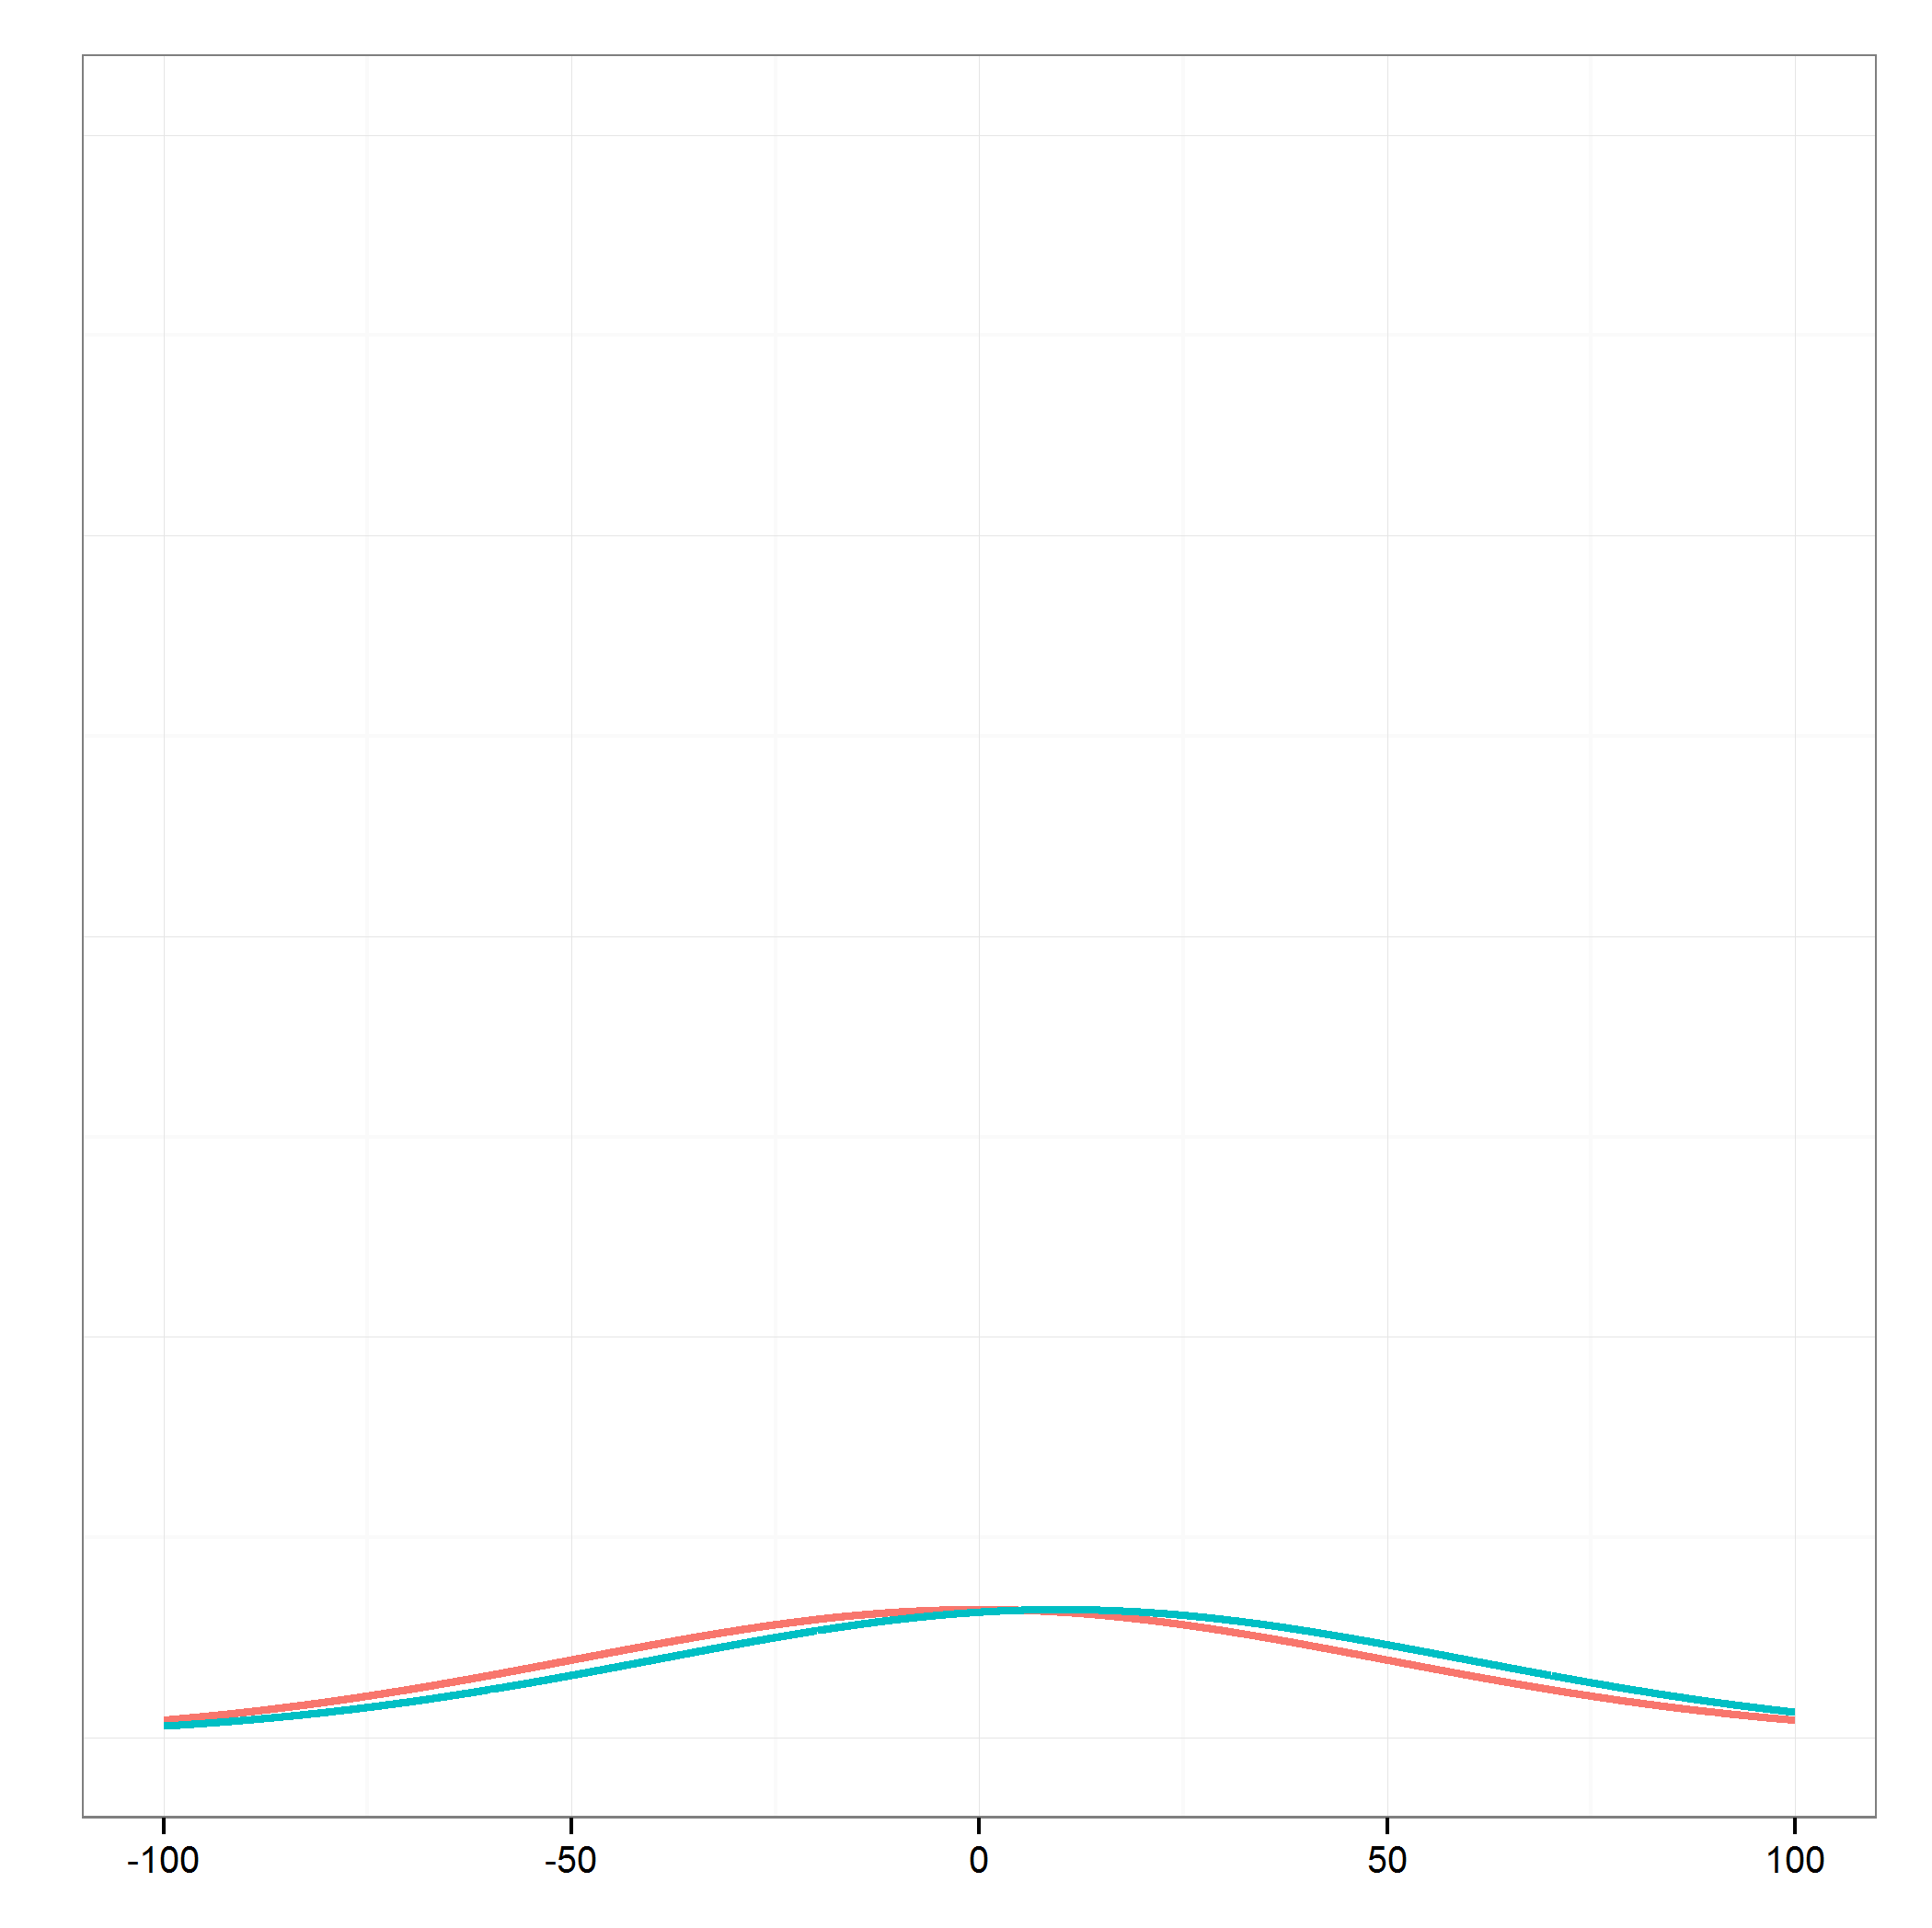
\includegraphics[scale=.3]{figs/first}
\end{block}
\end{column}%
\hfill%
\uncover<2->{
\begin{column}{.48\textwidth}
\begin{block}{\small Low Euclidean distance, High Distribution similarity}
{\small
$\mu_1=0,\sigma_1=0.01$\\
$\mu_2=0.1,\sigma_2=0.01$
}
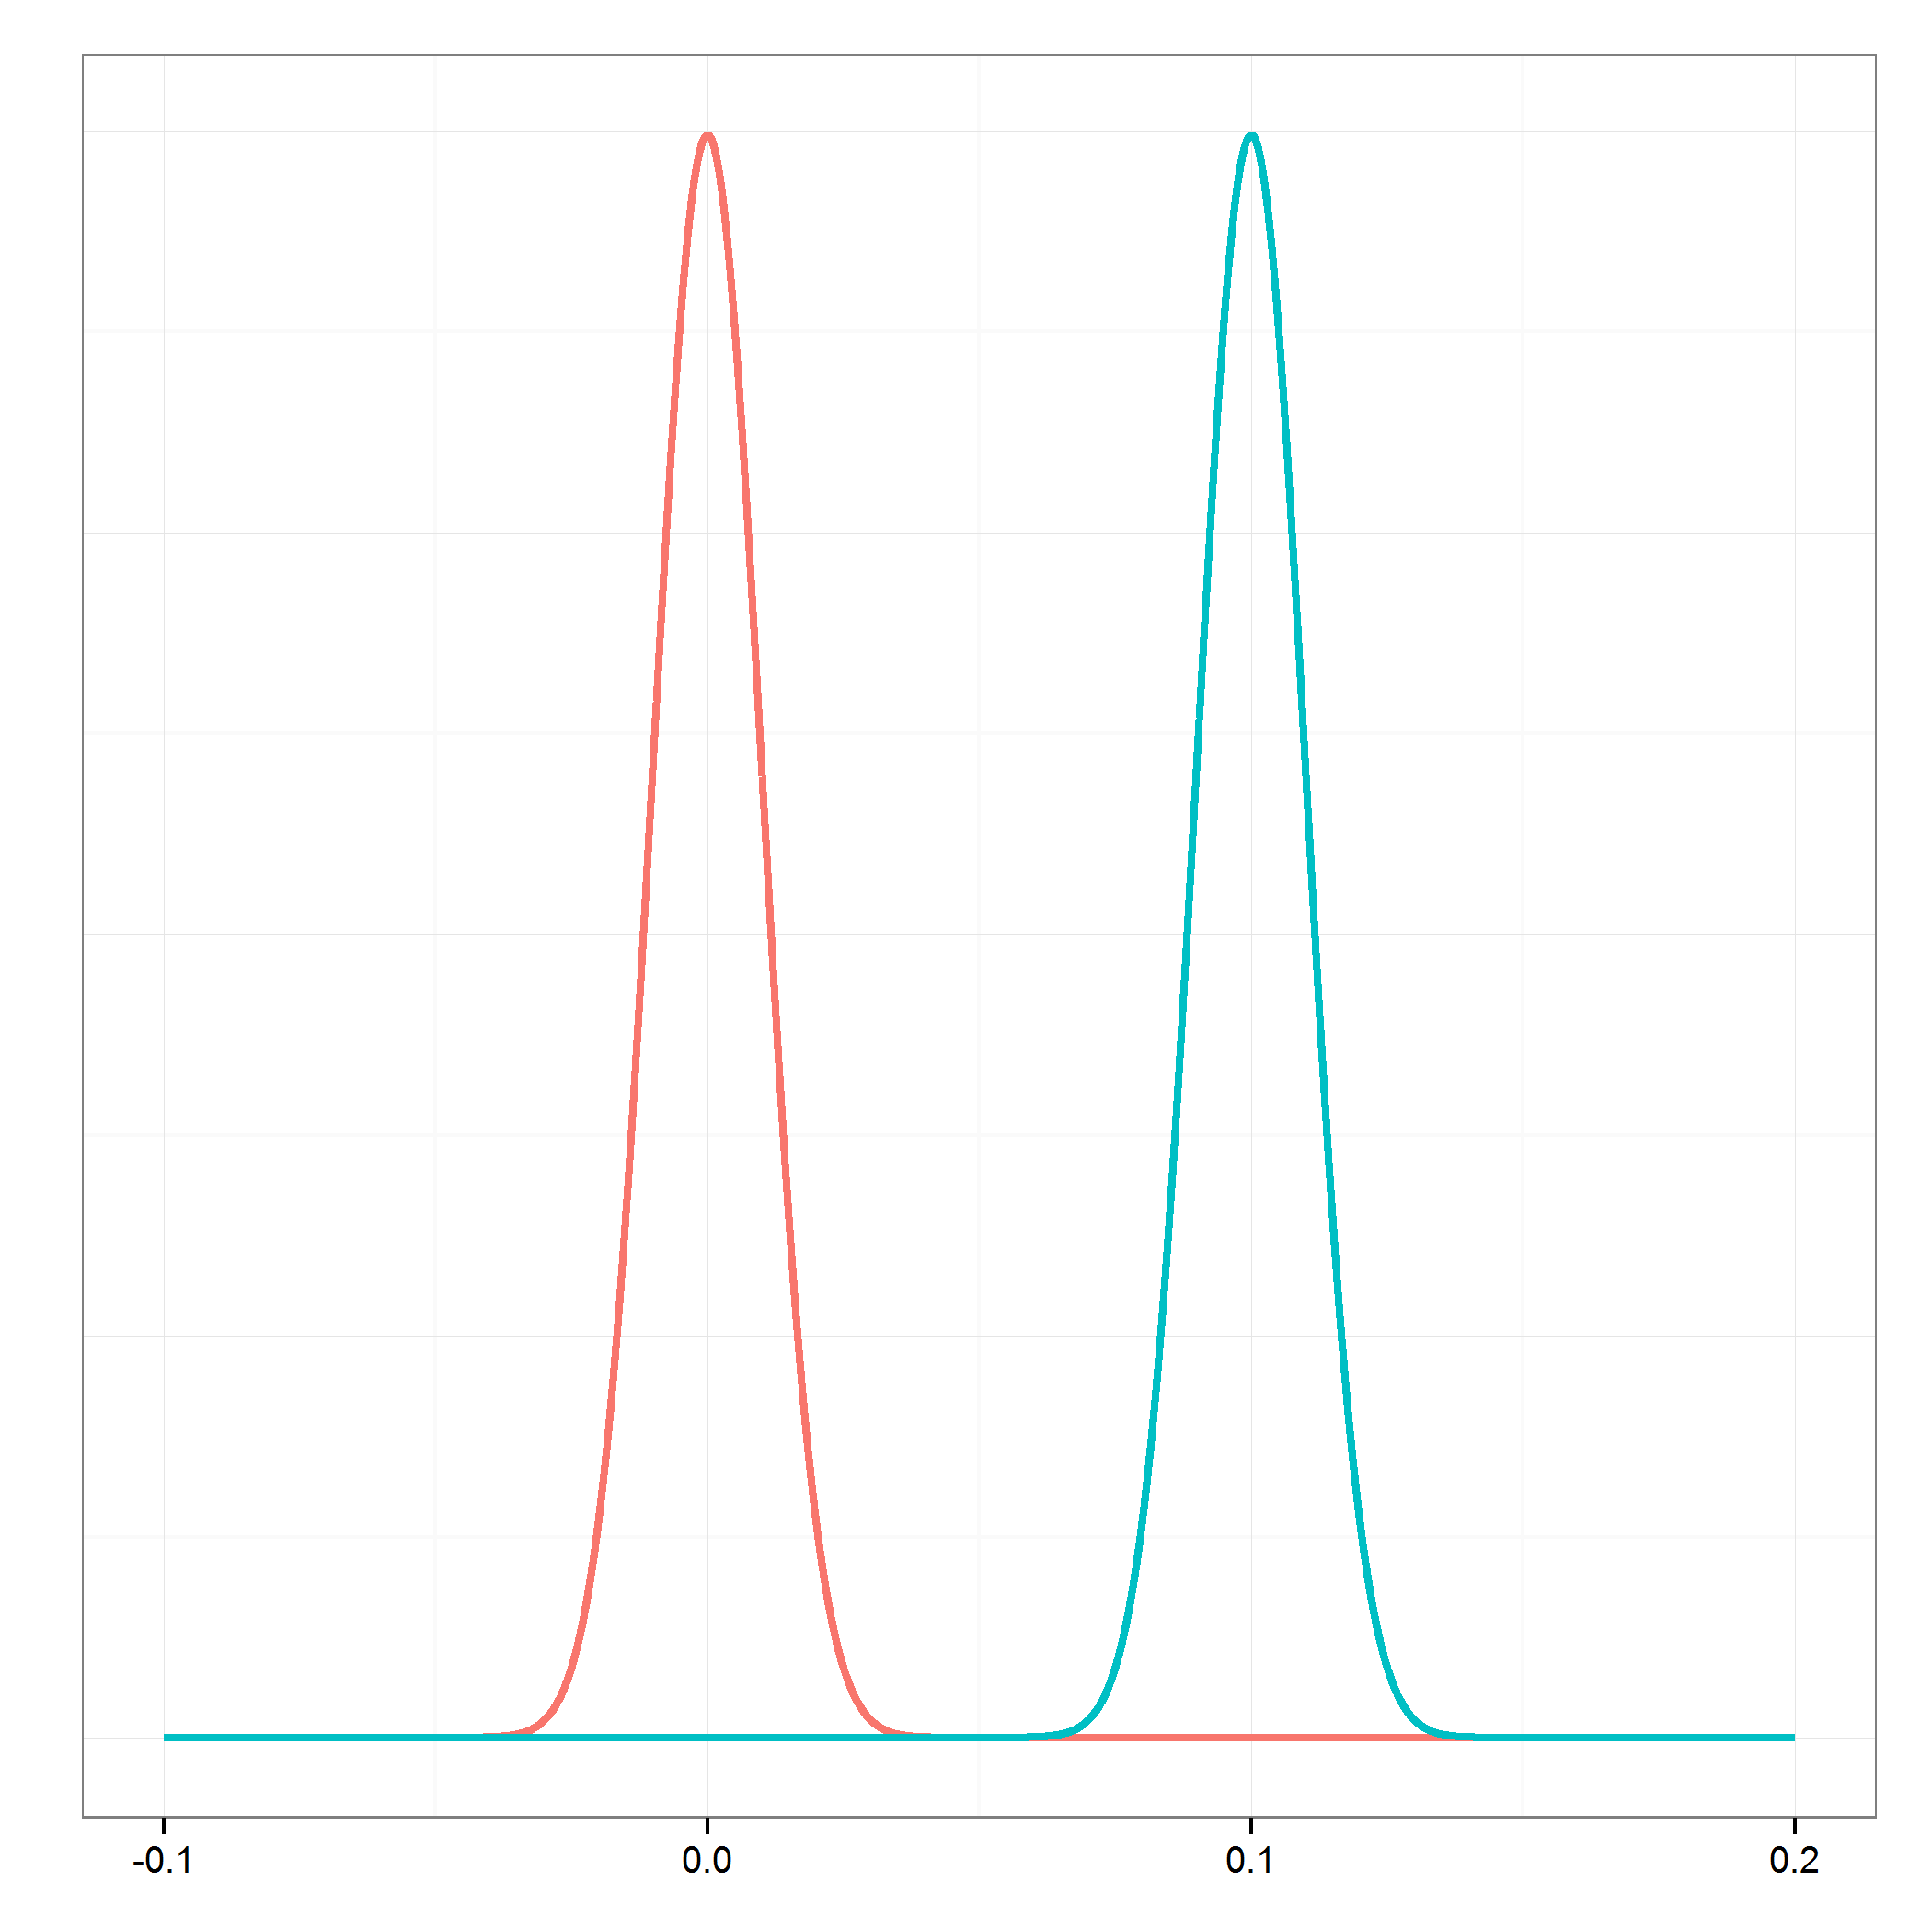
\includegraphics[scale=.3]{figs/second}
\end{block}
\end{column}%
}
\end{columns}
%%%%%%%%%%
}
\frame{\frametitle{``Close'' distributions $\approx$ small $D^{\textrm{sym}}_{KL}$}
\begin{itemize}
\item  $D^{\textrm{sym}}_{KL}(\lambda_0,\lambda_1) = 
\mathbb{E}_{\lambda_0}\left[ \log{\frac{p_{\lambda_0}}{p_{\lambda_1}} } \right] + 
\mathbb{E}_{\lambda_1}\left[ \log{\frac{p_{\lambda_1}}{p_{\lambda_0}} }\right]$
\item<2-> $p_1 \sim \mathcal{N}(\mu_1,\sigma_1)$, $p_2 \sim \mathcal{N}(\mu_2,\sigma_2)$
\end{itemize}
\uncover<3->{
\begin{columns}
\begin{column}{.48\textwidth}
\begin{block}{\small Similar distributions, Low $D^{\textrm{sym}}_{KL}$}
{\small
$\mu_1=0,\sigma_1=10K$\\
$\mu_2=10,\sigma_2=10K$\\
$D^{\textrm{sym}}_{KL} = 0.01$\\
}
\begin{center}
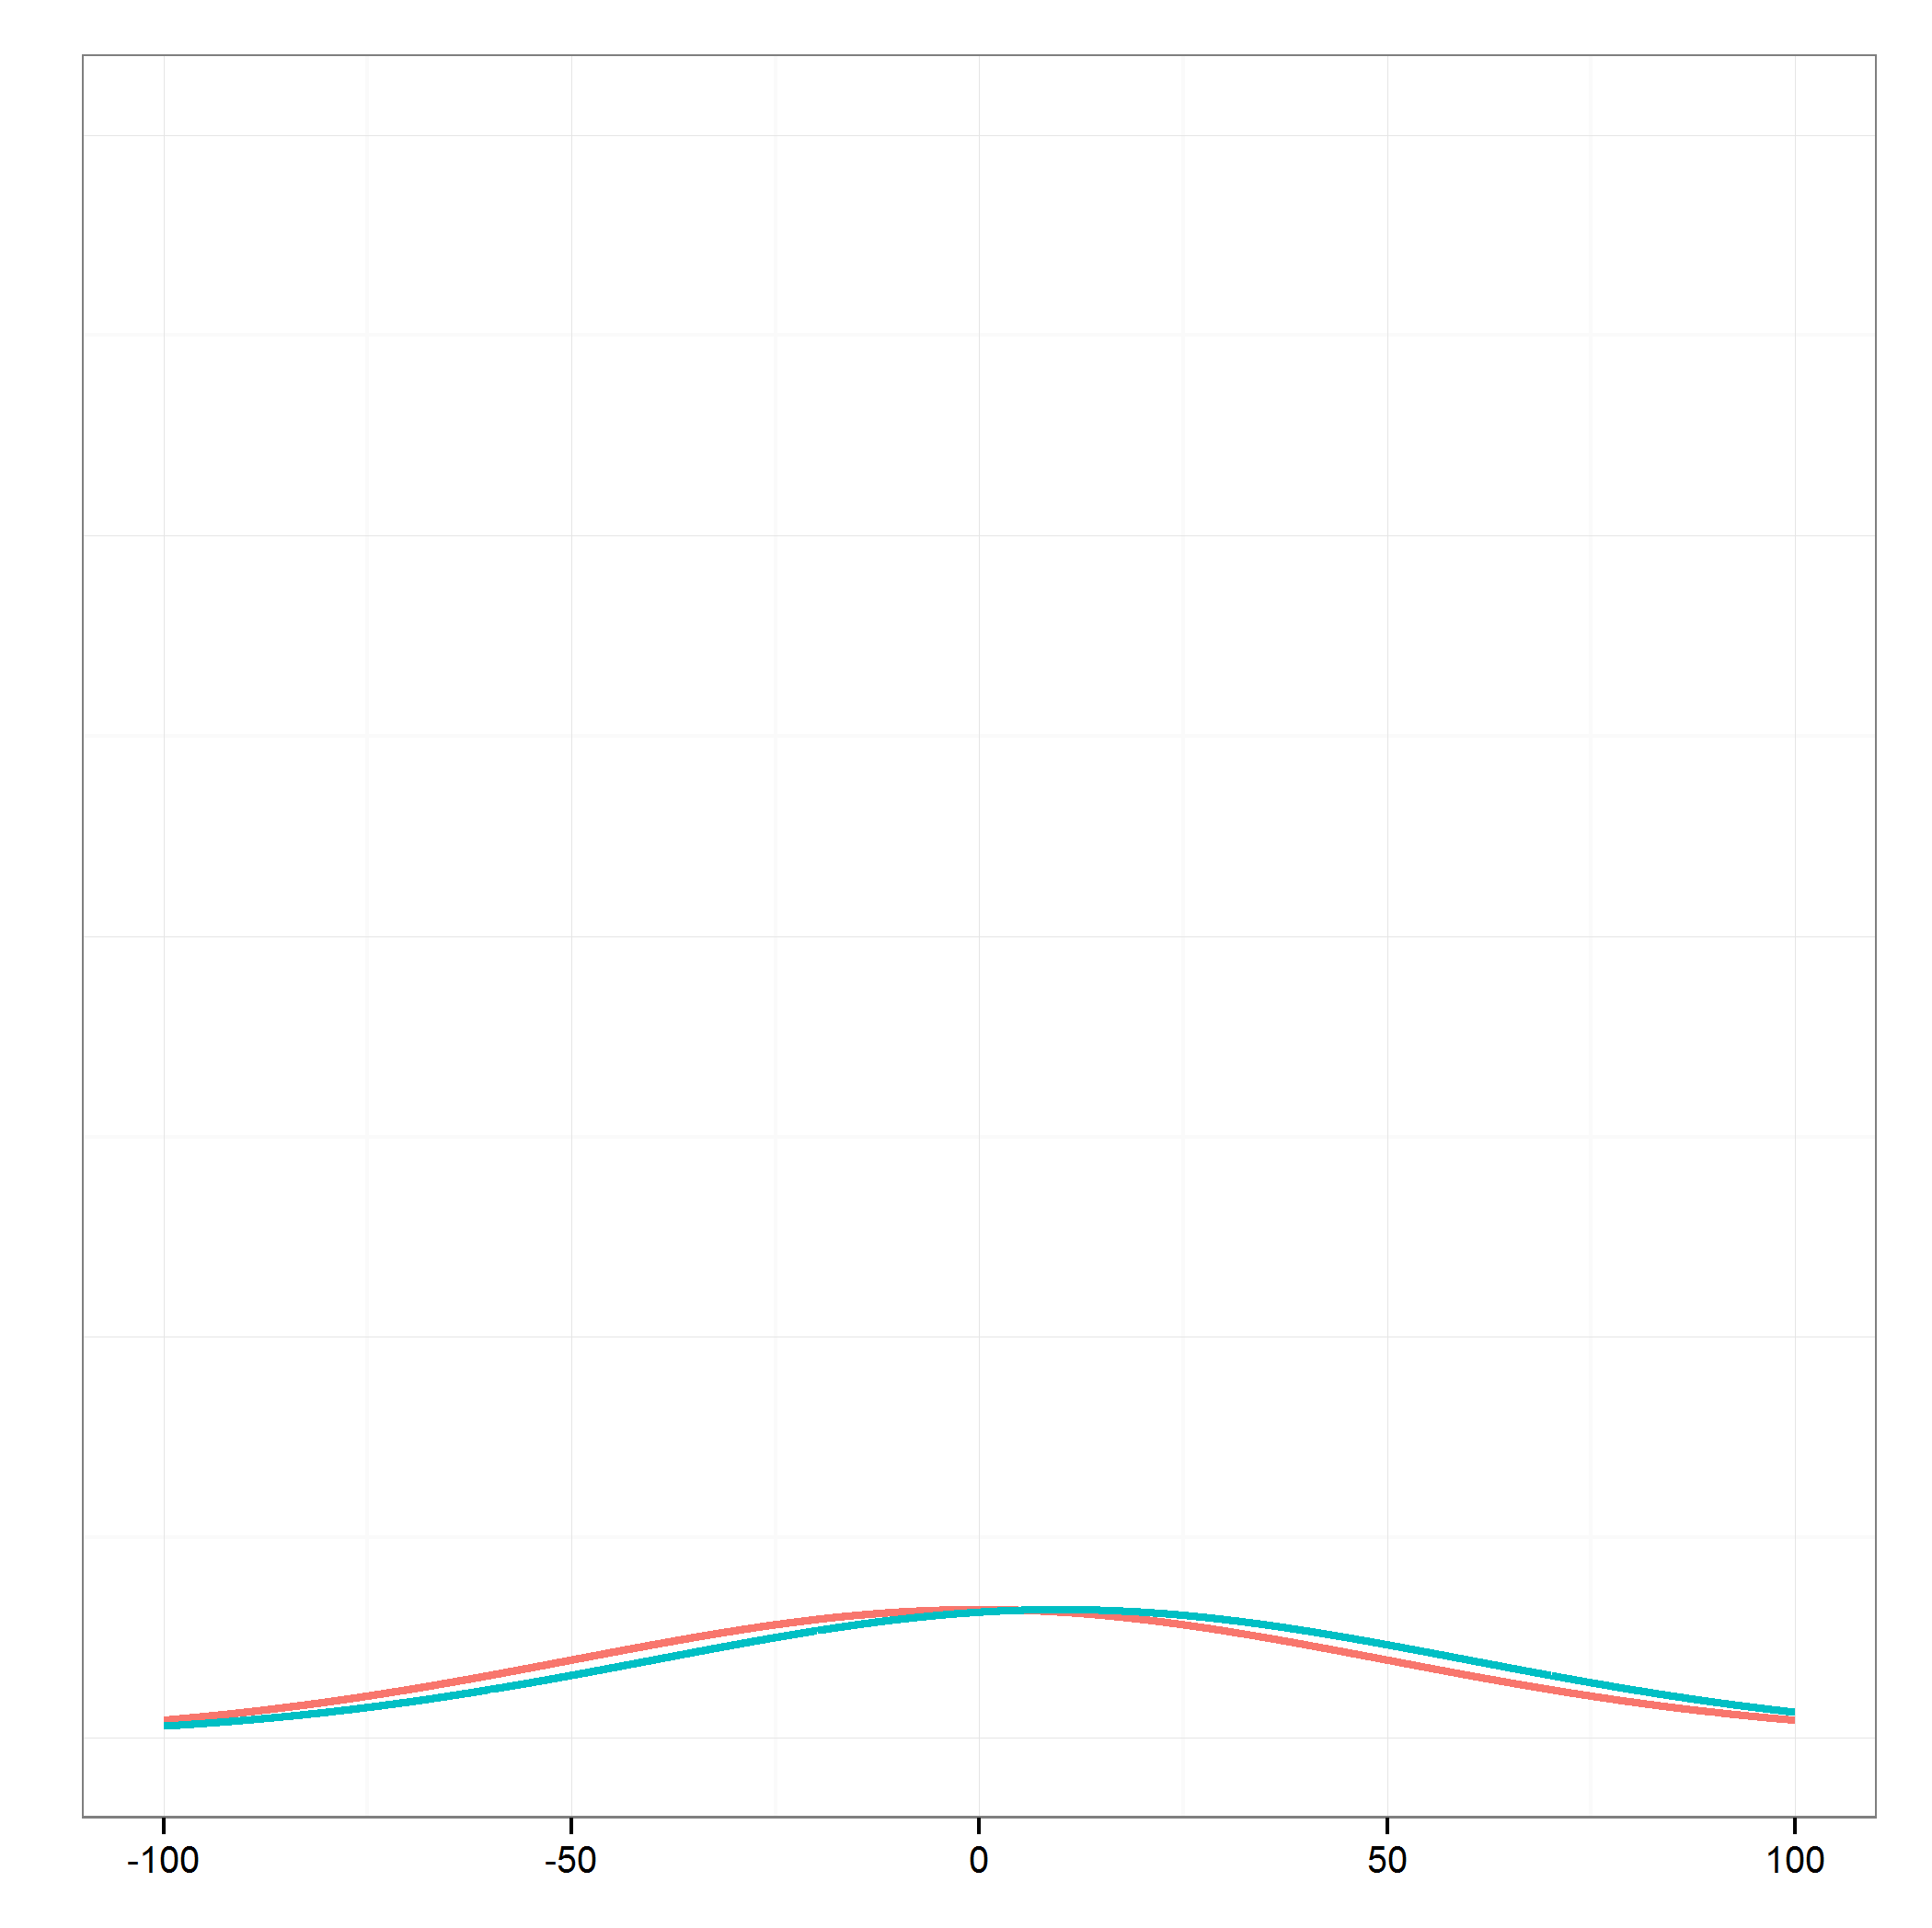
\includegraphics[scale=.2]{figs/first}
\end{center}
\end{block}
\end{column}%
\hfill%
\uncover<4->{
\begin{column}{.48\textwidth}
\begin{block}{\small Dissimilar distributions, High $D^{\textrm{sym}}_{KL}$}
{\small
$\mu_1=0,\sigma_1=0.01$\\
$\mu_2=0.1,\sigma_2=0.01$\\
$D^{\textrm{sym}}_{KL} = 1$\\
}
\begin{center}
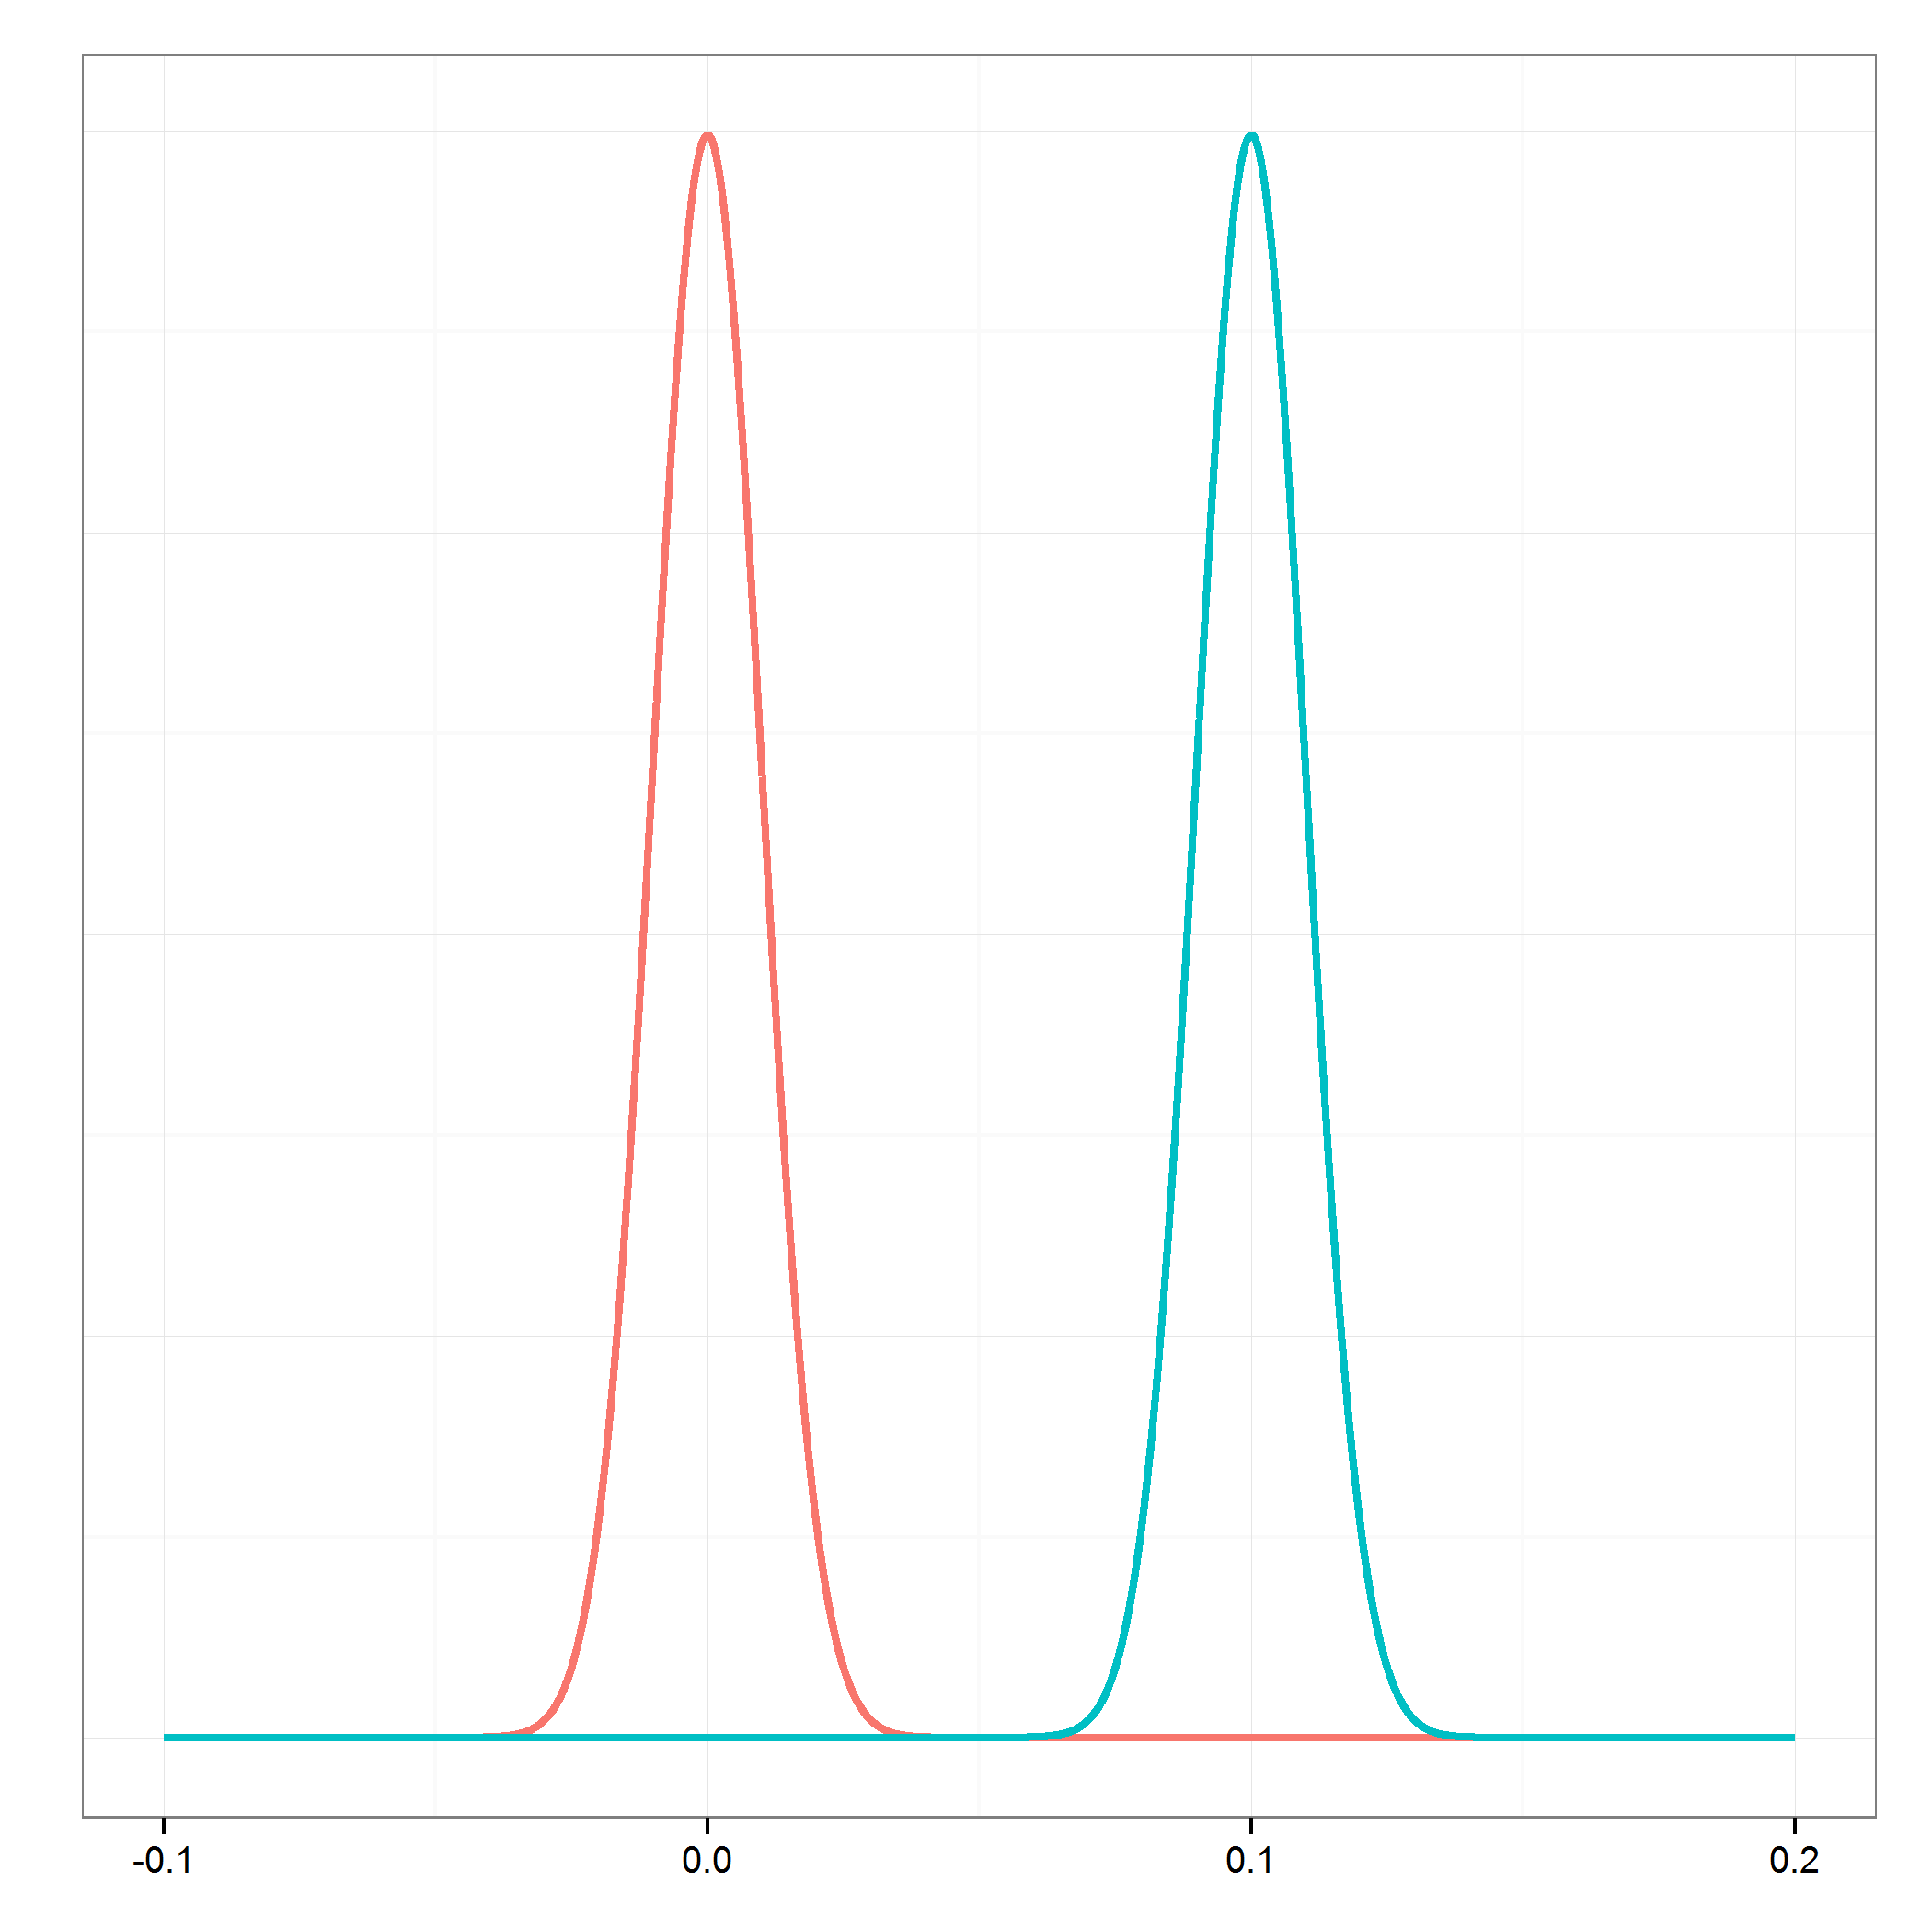
\includegraphics[scale=.2]{figs/second}
\end{center}
\end{block}
\end{column}%
}
\end{columns}
}
%%%%%%%%%%
}
\frame{\frametitle{Natural Gradient}
\begin{itemize}
\item Perform coordinate ascent according to a different metric
\uncover<2->{
\begin{align*}
\arg \max f(\lambda + d\lambda) & \textrm{ subject to } & 
\alt<3->{ D^{\textrm{sym}}_{KL}(\lambda, \lambda+d\lambda) < \epsilon}{\|d\lambda\|^2 < \epsilon^2}
\end{align*}
}
\item<4-> $D^{\textrm{sym}}_{KL} \approx d\lambda^\intercal G(\lambda) d\lambda$ for Riemannian metric $G$
\item<5-> Define the \textit{natural gradient} 
\begin{align*}
\hat \nabla_\lambda f(\lambda) 
\uncover<6->{& = & }
\uncover<7->{\redub{G(\lambda)^{-1}}_{\text{Inverse Fisher matrix}} \cdot}
\uncover<6->{ \redub{\nabla_\lambda f(\lambda)}_{\text{Euclidean gradient}}}
\end{align*}
\end{itemize}
}

\frame{\frametitle{Natural Gradient for mean field}
\begin{itemize}
\item Natural gradient: 

\begin{center}
$\hat \nabla_\lambda f(\lambda) = \redub{G(\lambda)^{-1}}_{\text{Inverse Fisher matrix}} \cdot \redub{\nabla_\lambda f(\lambda)}_{\text{Euclidean gradient}} $
\end{center}
\item<2-> ELBO gradient
\begin{center}
\begin{align*}
\nabla_\lambda \mathcal{L} 
& = & \nabla_\lambda^2 A_g(\lambda) \cdot \left(\mathbb{E}_q[ \eta_g(x,z,\alpha)] - \lambda\right) \\
\uncover<3->{& = & G(\lambda) \cdot \left(\mathbb{E}_q[ \eta_g(x,z,\alpha)] - \lambda\right) \\}
\end{align*}
\end{center}
\end{itemize}
}